\section{Results}

\subsection{Benchmark of values}

\begin{itemize}

  \item \textbf{Image: gain VS time for one single point. Overlay between
    experiment/daniels sim/our sim}

  \item comparison with previous values from Daniel's thesis

  \item (comparison with results from an experiment)

\end{itemize}



\subsection{Runtimes}
In Figure \ref{plot:runtime}, the developed parallel ASE-flux algorithm was compared to 
the original single threaded algorithm by Daniel Albach
\cite{ASE2010}. The mesh was sampled with different number of rays per sample
to show linear scaling of the algorithm. Using four GPUs, a speedup of up to 
296 (84 for one GPU) was reached. However, the GPU algorithm was enhanced with
more feature during development process, resulting more complex computations.
\begin{figure}[H]
  \centerline{
    \resizebox{0.5\textwidth}{!}{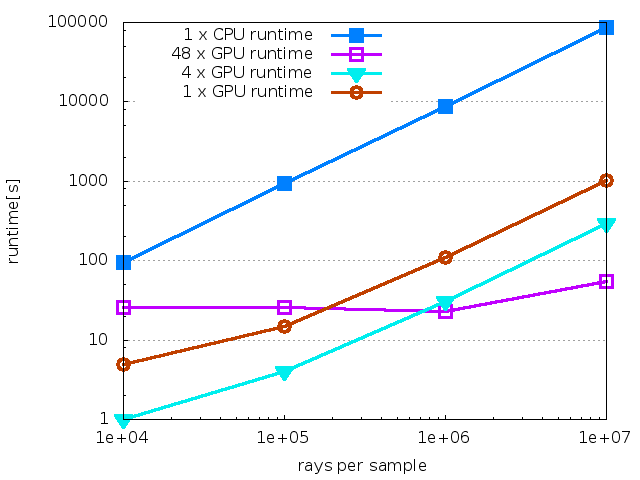
\includegraphics[width=8cm]{plot/runtime.png}}}
  \caption{Comparision implementation}
  \label{plot:runtime}
\end{figure}
Distributing the computation to multiple devices scales well up to the
point, that every sample point is simulated with the exact same number
of rays. Changing this (e.g. through adaptive sampling) leads to
a potencial unbalanced distribution of computation and therefore to
a worse scaling.

\begin{itemize}

  \item adaptive number of rays MUCH faster than fixed number of rays

  \item \textbf{Image: runtime VS precision of simulation} (precision based on
    MSE)

  \item use MSE to adjust the precision of the simulation rather than
    increasing the default number of rays

  \item law of diminishing returns: to lower the MSE below a certain threshold,
    exponentially more rays are required

  \item very low computation times result in values comparable to extremly long
    simulations.

  \item distributing the computation to multiple devices scales well
  \item \textbf{Image: GPU scaling with and without adaptive}

\end{itemize}
